\documentclass[12pt]{article}
\PassOptionsToPackage{quiet}{fontspec}
\usepackage[a4paper, total={6.5in, 10in}]{geometry}
\usepackage{amsmath}
\usepackage{amsfonts}
\usepackage{bm}
\usepackage{enumerate}
\usepackage{tikz}
\usepackage{ctex}
\usepackage{pgfplots}
\pgfplotsset{compat=1.17}
\usepackage{xcolor}
\usepackage{float}
\usepackage{booktabs}
\usepackage{graphicx}
\usepackage{latexalpha2}
\usepackage{framed}
\usepackage{verbatim}
\usepackage{listings}
\usepackage{latexalpha2}



\title{Test \LaTeX{} $\alpha_2$  in ArchLinux}
\date{\today}
\author{Eureka}
\begin{document}
\maketitle

\section{GNU Plot对比}
因为我们之前也说过,我们可以使用GNU Plot作为绘图的程序,以此来弥补TeX内部计算能力不足的问题。
当我们绘制点比较密集的函数,比如 $f(x)=x\sin(x)$, 
tik{\bf 会自己}调用外部的GNU Plot(在你允许的情况下)下面就是一个例子:

\begin{center}
	\begin{tikzpicture}
		\begin{axis}[axis x line = middle,
		axis y line = middle,
		xmin=-20, xmax=30,
		ymin=-350, ymax=70]
		\addplot[domain=-12:26,color=orange,very thick,smooth]
			gnuplot {14*x-x^2};
		\end{axis}
	\end{tikzpicture}
\end{center}


\newcommand{\ploT}[2][red]{
	\begin{tikzpicture}
		\begin{axis}[axis x line = middle,
		axis y line = middle,
		xmin=-20, xmax=20,
		ymin=-20, ymax=20]
		\addplot[domain=-5:5,color=#1,thick,smooth]
			gnuplot {#2};
		\end{axis}
	\end{tikzpicture}
}
\ploT{sin(x)*exp(x) + 2*x}

然而下面这个命令就没有用到GNU Plot,导致绘制这幅图的花费时间大幅上升
% \begin{center}
% 	\plotz{}{sin(deg(sqrt(x^2+y^2)))/sqrt(x^2+y^2)}{surf}{}{图例}
% \end{center}

或者是使用GNU Plot 生成三维图像:

\begin{center}
	\begin{tikzpicture}
	\begin{axis}
		\addplot3[surf, domain=-2:2, domain y=-2:2, raw gnuplot] 
			gnuplot {
				f(x, y) = sin(x) * cos(y);
				splot f(x, y);
			};
	\end{axis}
	\end{tikzpicture}
\end{center}

\begin{center}
	\begin{tikzpicture}[scale=2]
		\begin{axis}[view={60}{30},axis equal image]
		\addplot3 [
			contour gnuplot={
			contour dir=x,
			number=20,
			labels=false,
		},
		samples=50,domain=-1:1,y domain=0:2*pi,
		] (
			{sqrt(1-x^2) * cos(deg(y))},
			{sqrt( 1-x^2 ) * sin(deg(y))},
			x
		);
		\end{axis}
	\end{tikzpicture}
\end{center}

\newcommand{\plotZ}[1]{
	\begin{tikzpicture}
	\begin{axis}[colormap/cool]
		% raw gnuplot选项用于在\addplot命令中直接使用Gnuplot命令。
		% 它允许您以Gnuplot语法编写绘图函数,而不需要转换为TikZ函数。
		\addplot3[surf,raw gnuplot]gnuplot {
			f(x, y) = #1;
			splot f(x, y);
		};
	\end{axis}
	\end{tikzpicture}
}

测试

\begin{center}
	\plotZ{x*y}
\end{center}

% \begin{tikzpicture}
% 	\begin{axis}[colormap/cool]
% 		% raw gnuplot选项用于在\addplot命令中直接使用Gnuplot命令。
% 		% 它允许您以Gnuplot语法编写绘图函数,而不需要转换为TikZ函数。
% 		\addplot3[surf, raw gnuplot] gnuplot {
% 			f(x, y) = x*y;
% 			splot f(x, y);
% 		};
% 	\end{axis}
% \end{tikzpicture}
	



但是GNU Plot还是不太灵活的,下面我们考虑\LaTeX{} 和MMA联合,在\LaTeX{} 
的内部调用MMA绘图,以及计算等大部分的功能.




\section{引入latexalpha2宏包}
引入 \LaTeX{}$\alpha_2$  宏包的安装是十分的简单的,只需要我们把sty文件放到对应的.tex目录下即可。

\section{宏包使用}
一个简单的测试MMA和\LaTeX{} 联合样例:

\begin{align}
    \wolfram{Series[Exp[x], {x, 0, 5}]}
\end{align}
 
 可以成功,只不过跨系统调用有一点点的慢。
这个宏包提供的命令有如下:

\begin{framed}
\begin{itemize}
    \item \verb|\wolfram[<format>]{<code>}|:在花括号\{\}中传入MMA的命令即可
    \item \verb|\wolframgraphics[<format>]{<code>}{<filename>}|:先给出绘制的图片名,后面使用\verb|\includegraphics{}|调用
    \item \verb|\wolframsolve{<equation>}{<variable>}|:解关于变量<variable>的方程
    \item \verb|\wolframdsolve{<equation>}{<dependent variable>}{<independent variable>}|:求解微分方程
    \item \verb|\wolframtex{<format>}{<code>}|:输入\LaTeX{} 格式的MMA代码求解
    \item \verb|\wolframanimation{<code>}{<foldername>}|:使用MMA创建动画,注意只有部分的pdf阅读器支持pdf中内嵌动画
    \item \verb|\wolframtable{<table>}|:把一个MMA中的表格转化为\LaTeX{} 格式,可以嵌入到{\ttfamily tabular, tabularx}等环境中\ttfamily tabular, tabularx
\end{itemize}
\end{framed}

\subsection{Using \LaTeX $\alpha_2$ to include graphics}


\begin{figure}[!htb]
	\centering
    \wolframgraphics{Plot3D[Sin[x]*Cos[y],{x,-2Pi,2Pi},{y,-2Pi,2Pi}]}{example}
    \wolframgraphics{ComplexPlot3D[(z^2+1)/(z^2-1),{z,-2-2 I,2+2 I},PlotLegends->Automatic,AxesStyle->Arrowheads[{0,0.03}]]}{ComplexPlot3D}
	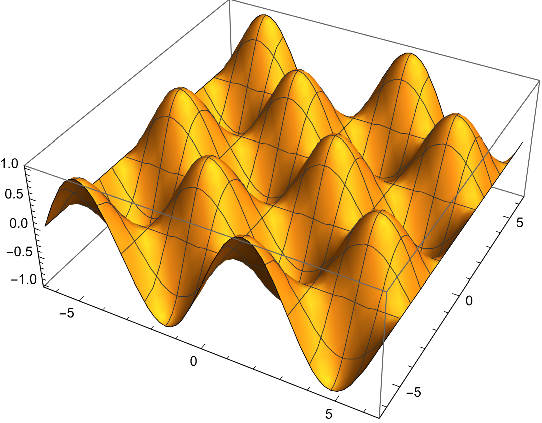
\includegraphics[scale=.7]{example.pdf}
	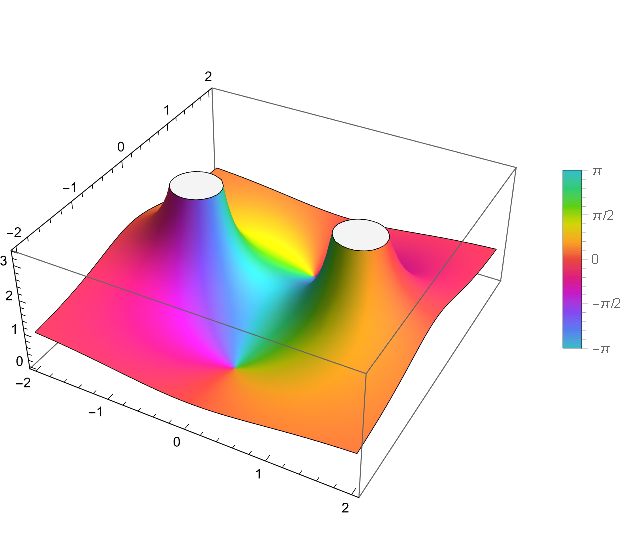
\includegraphics[scale=.7]{ComplexPlot3D.pdf}
	\caption{图片测试}
	\label{图片测试}
\end{figure}


一个复杂的绘制函数的例子,我们首先定义了一个函数,然后便是绘制了一个用于测试的函数,
结果是不可行的。

经过实际测试,行不通。但是可以把这个绘制命令写的复杂一点,我们绘制了一个定义了一系列命令的二维
函数绘制例子,定义了它的颜色,比例,标签,刻度等。

\begin{figure}[!htb]
    \centering
    \wolframgraphics{
		ContourPlot[
		x^2/4 + y^2/3 == 5, {x, -5, 5}, {y, -5, 5},
		ContourStyle->{
			% 同样的,被latex注释的部分不会传入MMA
			% RGBColor["\#00C0A3"], 
			% 在传参的过程中,不要使用#,即使是\#,MMA也是会报错的。
			RGBColor[0.,0.7529411764705882,0.6392156862745098],
			Thickness[0.004]
		},
		AspectRatio->1, 
		AxesOrigin->{0,0}, 
		Axes->True,
		Frame->False,
		AxesStyle->Arrowheads[{0, 0.03}],
		AxesLabel->{"x", "y"}
	]}{ComplexCmd}
    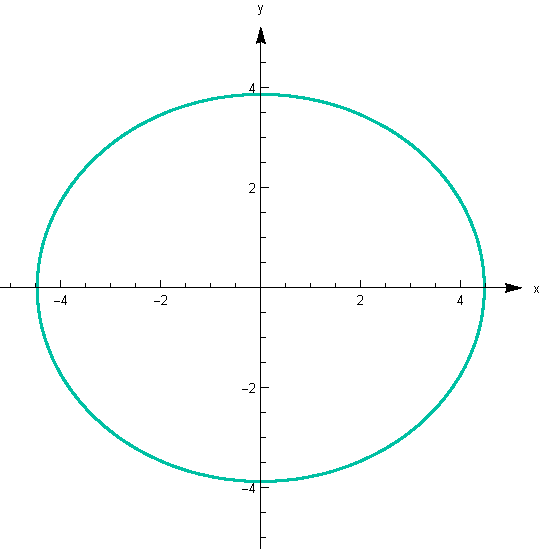
\includegraphics[scale=.7]{ComplexCmd.pdf}
	\caption{复杂命令测试}
	\label{复杂命令测试}
\end{figure}


\clearpage
\section{命令封装}
下面我们把命令封装在一起,方便以后调用

% \newcommand{\test}[3]{
% 	\begin{figure}[!htb]
% 		\centering
% 		\wolframgraphics{
% 			ContourPlot[
% 			x^2/4 + y^2/3 == 5, {#1}, {#2},
% 			ContourStyle->{
% 				RGBColor[0.,0.7529411764705882,0.6392156862745098],
% 				Thickness[0.004]
% 			},
% 			AspectRatio->1, 
% 			AxesOrigin->{0,0}, 
% 			Axes->True,
% 			Frame->False,
% 			AxesStyle->Arrowheads[{0, 0.03}],
% 			AxesLabel->{"x", "y"}
% 		]}{#3}
% 		\includegraphics[scale=.7]{#3}
% 		\caption{#3}
% 		\label{#3}
% 	\end{figure}
% }



% \begin{test}{{x, -5, 5}}{{y, -5, 5}}{Test3}

% \end{test}
% \test{{x, -5, 5}}{{y, -5, 5}}{Test3}


% \newcommand{\testa}{
% 	\begin{figure}[!htb]
% 		\centering
% 		\wolframgraphics{
% 			ContourPlot[
% 			x^2/4 + y^2/3 == 5, {x, -5, 5}, {y, -5, 5},
% 			ContourStyle->{
% 				% 同样的,被latex注释的部分不会传入MMA
% 				% RGBColor["\#00C0A3"], 
% 				% 在传参的过程中,不要使用#,即使是\#,MMA也是会报错的。
% 				RGBColor[0.,0.7529411764705882,0.6392156862745098],
% 				Thickness[0.004]
% 			},
% 			AspectRatio->1, 
% 			AxesOrigin->{0,0}, 
% 			Axes->True,
% 			Frame->False,
% 			AxesStyle->Arrowheads[{0, 0.03}],
% 			AxesLabel->{"x", "y"}
% 		]}{ComplexCmd2}
% 		\includegraphics[scale=.7]{ComplexCmd2.pdf}
% 		\caption{复杂命令测试2}
% 		\label{复杂命令测试2}
% 	\end{figure}
% }

% \testa


% \newcommand{\testb}[1]{
% 	\begin{figure}[!htb]
% 		\centering
% 		\wolframgraphics{
% 			ContourPlot[
% 			x^2/4 + y^2/3 == 5, {x, -5, #1}, {y, -5, 5},
% 			ContourStyle->{
% 				% 同样的,被latex注释的部分不会传入MMA
% 				% RGBColor["\#00C0A3"], 
% 				% 在传参的过程中,不要使用#,即使是\#,MMA也是会报错的。
% 				RGBColor[0.,0.7529411764705882,0.6392156862745098],
% 				Thickness[0.004]
% 			},
% 			AspectRatio->1, 
% 			AxesOrigin->{0,0}, 
% 			Axes->True,
% 			Frame->False,
% 			AxesStyle->Arrowheads[{0, 0.03}],
% 			AxesLabel->{"x", "y"}
% 		]}{ComplexCmd3}
% 		\includegraphics[scale=.7]{ComplexCmd3.pdf}
% 		\caption{复杂命令测试3}
% 		\label{复杂命令测试3}
% 	\end{figure}
% }

% \testb{5}


\newcommand{\testc}[1]{
	\begin{figure}[!htb]
		\centering
		\wolframgraphics{
			ContourPlot[
			x^2/4 + y^2/3 == 5, #1, {y, -5, 5},
			ContourStyle->{
				% 同样的,被latex注释的部分不会传入MMA
				% RGBColor["\#00C0A3"], 
				% 在传参的过程中,不要使用#,即使是\#,MMA也是会报错的。
				RGBColor[0.,0.7529411764705882,0.6392156862745098],
				Thickness[0.004]
			},
			AspectRatio->1, 
			AxesOrigin->{0,0}, 
			Axes->True,
			Frame->False,
			AxesStyle->Arrowheads[{0, 0.03}],
			AxesLabel->{"x", "y"}
		]}{ComplexCmd4}
		\includegraphics[scale=.7]{ComplexCmd4.pdf}
		\caption{复杂命令测试4}
		\label{复杂命令测试4}
	\end{figure}
}

% \testc{{x, -5, 5}}



% \newcommand{\mycommand}[1]{%
%     % 在这里可以使用传递进来的参数
%     参数值为:#1
% }

% % 在文档中调用自定义命令,并传递参数 {x, -5, 5}
% \mycommand{{x, -2, 8}}


\end{document}
